Rayleigh fading is generated by a standard complex gaussian.
\begin{equation*}
    h \sim \mathcal{CN}(0, 1)
\end{equation*}
The four combining technique are implemented and the results are shown below:
\begin{itemize}
    \item[(a)] \textbf{Selective Combining (SC)} \hfill \\
    Choose the \textcolor{blue}{strongest branch} as the combining result.
    \begin{figure}[H]
        \centering
        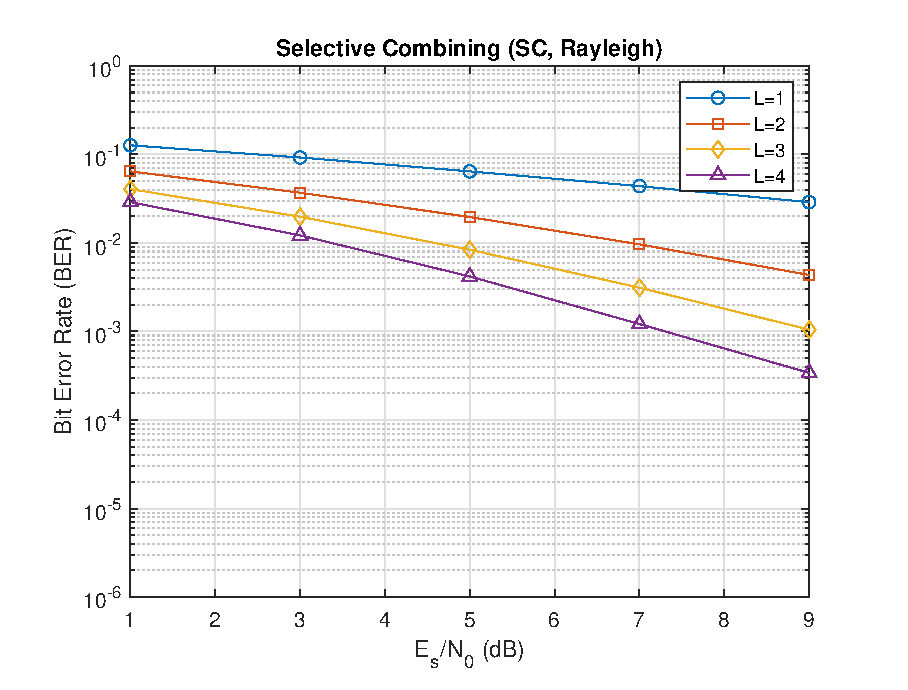
\includegraphics[scale = 0.85]{SC_rayleigh.eps}
    \end{figure}
    \vfill
    \item[(b)] \textbf{Maximal Ratio Combinig (MRC)} \hfill \\
    Weight each branch according to the \textcolor{blue}{corresponding channel gain.}
    \begin{figure}[H]
        \centering
        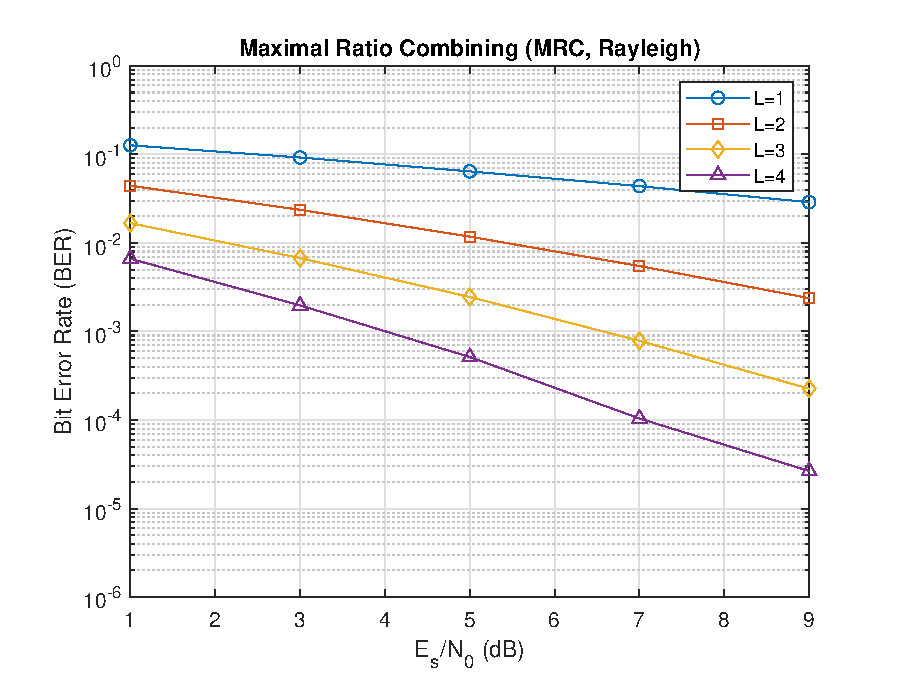
\includegraphics[scale = 0.85]{MRC_rayleigh.eps}
    \end{figure}
    \item[(c)] \textbf{Equal Gain Combinig (MRC)} \hfill \\
    Weight each branch with \textcolor{blue}{same gain.}
    \begin{figure}[H]
        \centering
        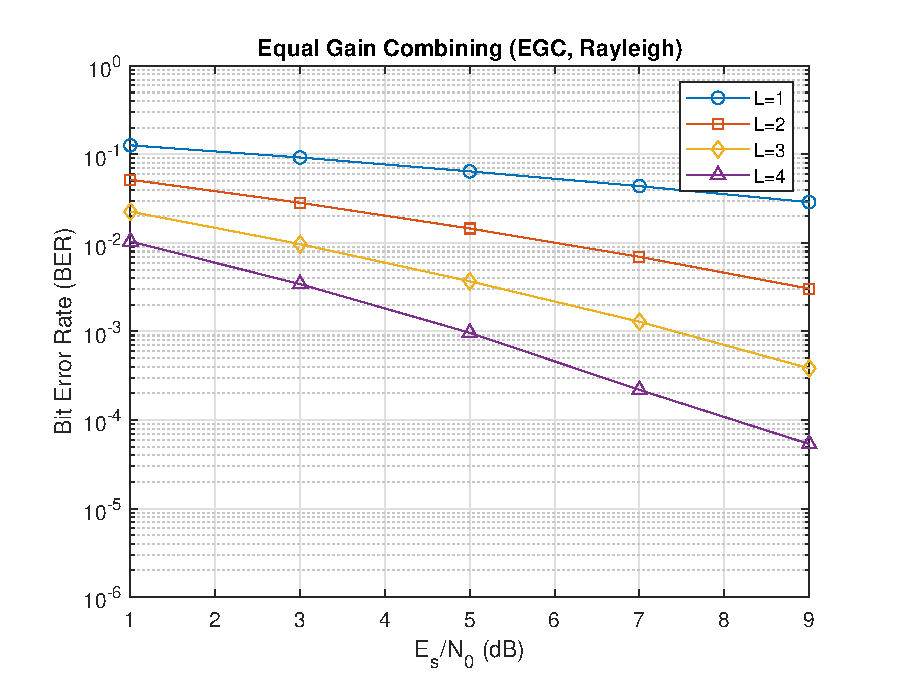
\includegraphics[scale = 0.85]{EGC_rayleigh.eps}
    \end{figure}
    \item[(d)] \textbf{Direct Combinig (MRC)} \hfill \\
    Combine each branch directly and then compensate phase.
    \begin{figure}[H]
        \centering
        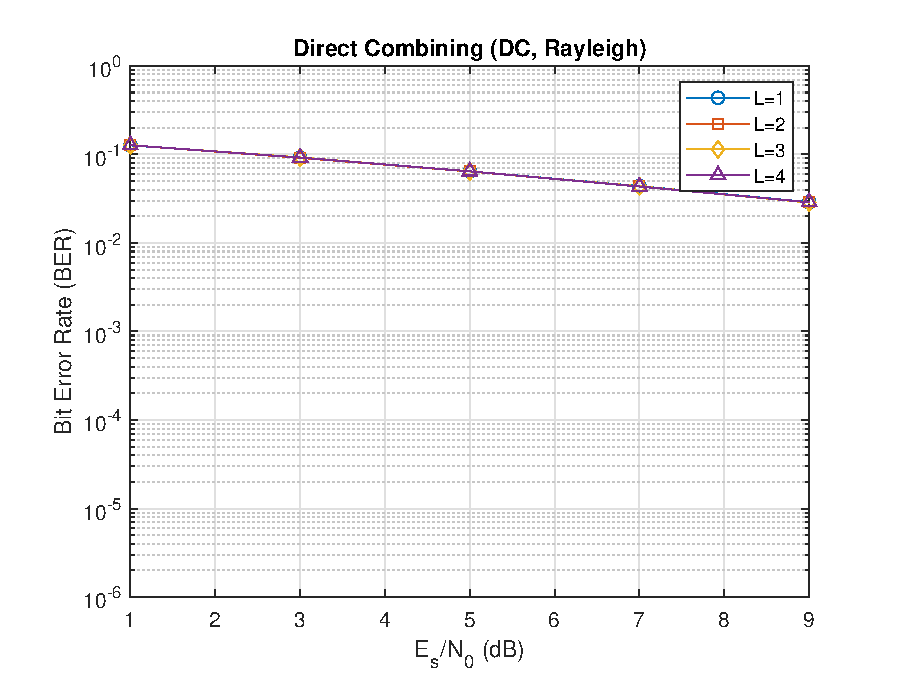
\includegraphics[scale = 0.85]{DC_rayleigh.eps}
    \end{figure}
\end{itemize}